\chapter{Timers} \label{CHAP:TIMERS}

\section{Motivation: Why Timers?}

Examples where timers are needed:
\begin{itemize}
\item repetitive tasks of
	\begin{itemize}
	\item the client: VoIP, multimedia player, ...
	\item the server: refresh of pages, speed for streaming, ...
	\end{itemize}
\item timeouts
\item scheduling
\item flow control
\item message acknowledgements
\item failure recovery
\end{itemize}
$\Rightarrow$ a large number of timers with fine granularity is needed

\section{Different timers}

Precondictions: 
\begin{itemize}
\item the maximum possible interval is known (given by the storage used for an interval, e.g. $32$ bit results in maximum interval $2^{32}$)
\item the intervals are represented by integers
\end{itemize}

Supported operations:
\begin{itemize}
\item startTimer(interval, id, expiryAction): inserts the timer
\item stopTimer(id): removes the timer
\item perTickBookkeeping(): checks for expired timers (and calls stopTimer(id))
\item expiryProcessing(): calls the expiryAction-method
\end{itemize}

\subsection{Timing Wheels}

General idea: hash the timers into buckets with their interval as key.

\subsubsection{Hashed Wheels}

Idea: the first $x$ bits are hashed into buckets, the remainder is inserted into a sorted linked list.\\

Costs refer to the worst-case running time for one method call, where $n$ is the overall number of timers and $n(t) \leq n$ denotes the number of expired timers at the moment $t$.\\
\begin{tabular}{p{0.2\linewidth}|p{0.6\linewidth}|p{0.2\linewidth}}
Method & Action & Costs \\
\hline \hline
startTimer & hash the timer into a bucket using $x$ higher order bits of its interval; insert the timer into a sorted linked list (ordered by expiration) & $O(n)$ since we have to traverse the whole list\\
perTickBookkeeping & calculate the bucket of the current time; expire all timers in the list until we reach the first timer, that expires later; we can stop since the list is sorted & $O(n(t))$ which is optimal \\
\end{tabular}\\
For stopTimer we store a pointer to the timer and use a doubly linked list, then we can remove it in $O(1)$.\\

Conclusion: 
\begin{itemize}
\item fast perTickBookkeeping
\item slow insertion, especially if many timers are in one bucket and thus the sorted linked list is large
\end{itemize}

\subsubsection{Hierarchical Wheels}

Idea: use different arrays at different precision levels and look at the timer in detail only if you need to do so because it expires soon.\\
(Note that we can calculate how many levels we need, because we know the maximum interval that is possible.)\\

Example:\\
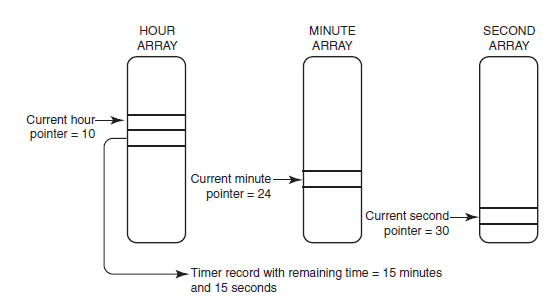
\includegraphics[width=0.5\linewidth]{images/chap7/hierarchicalTimingWheel.png}\\
To add a timer that expires in $5$ seconds, i.e. at $10:24:45$, we insert it directly into the Second Array.\\
To add a timer that expires in $3$ minutes, i.e. at $10:27:30$, we insert it into the Minute Array, since minutes is the highest level on which the value isn't equal to the current time.\\
When the current time points to $27$ all entries of this bucket are inserted into the Second Array.\\

\begin{tabular}{p{0.2\linewidth}|p{0.6\linewidth}|p{0.2\linewidth}}
Method & Action & Costs \\
\hline \hline
startTimer & hash the timer into the right bucket on the right level (highest level where current time and timer interval are not equal); insert it as first timer into the list of timers there & $O(1)$ which is optimal\\
perTickBookkeeping & expire and remove all timers in the current bucket at the lowest level; if the current time reached the end of an array, update levels from the next higher level (continue if necessary until highest level), i.e. take the current bucket and hash its timers to the lower level &  $O(n)$ since we have to traverse the lists of all levels in the worst-case and they may consist of all timers \\
\end{tabular}\\

Conclusion: 
\begin{itemize}
\item fast insertion
\item slower perTickBookkeeping, but only if the current time reaches the end of an array and every timer is touched maximal once for each level
\end{itemize}

Note: if precision of timers is allowed to decrease with higher levels, we don't have to update the timers into a different level.

\subsection{BSD implementation}

$200$ msec timers are used.\\

In the BSD implementation the method to stop the timer cannot take a pointer as argument.\\
Two possible solutions:
\begin{itemize}
\item define a new function which takes a pointer as argument
\item or use a hash table to search the callout for a given function
\end{itemize}

\subsection{Soft timers}

Problem: perTickBookkeeping can only be called as often as the timer ticks, thus we need fine granular timers. \\
Normal is around $1$ msec. If we want to achieve finer granularity, we could use a programmable harware interrupt chip (provided by most CPUs). But this causes a lot of overhead, ~$45$\%, because the CPU state (i.e. registers, TLB, ...) has to be stored on each interrupt.\\

Solution: Use other transition events, that include saving the CPU state anyway (e.g. system calls, exceptions, hardware interrupts), and add a timer interrupt there. \\
But we trade precision for speed, since usually such an event takes place every $10 \mu$sec, but it is not guaranteed.\\
In order to guarantee a worst-case of $1$ msec, we could add a hardware clock interrupt every $1$ msec.